\section{The Simple Unlinkable Protocol}
\label{sec:unlinkable-simple}

In considering a cryptographic approach to creating an Unlinkable Credit Card Protocol, let us first consider the simpler approach of using symmetric cryptography.
In a cryptographic scheme employing symmetric cryptography,
    the original sender (the credit card) and the final destination (the bank) share a secret key used for both encryption and decryption.
While symmetric cryptography can provide confidentiality of a message from the card to the bank, it cannot provide unlinkability.
This is because the message received by the bank must include some method for determining which of its customer's keys the bank should use to decrypt the message.
The retailer may then simply use this key identifier to link purchases.

Let us next consider using asymmetric (or ``public key'') cryptography,
  a system in which anybody (having access only to publicly available information) may encrypt a message that only the intended recipient may decrypt.
Asymmetric cryptography allows the recipient to use a single key in order to decrypt messages originating from any party, sidestepping the key identifier issue above.

We thus present the Simple Unlinkable Wallet Protocol, employing asymmetric encryption to maintain unlinkability.
This protocol is illustrated in Figure \ref{fig:simple-cpp}, and operates as follows:

\begin{figure}[h]
  \caption{Simple Unlinkable Wallet Protocol}
  \centering
    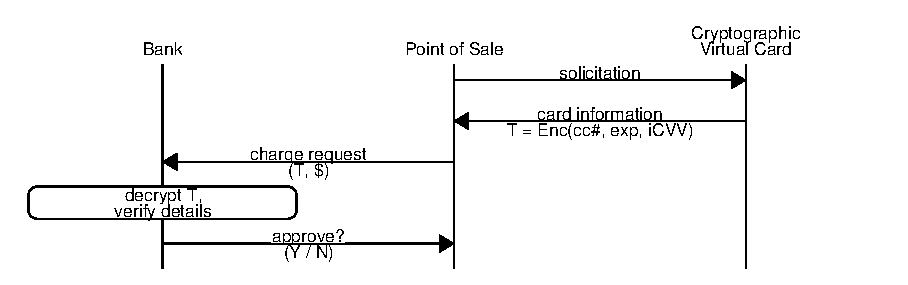
\includegraphics{img/simple-unlinkable-cpp.eps}
  \label{fig:simple-cpp}
\end{figure}

\begin{enumerate}
    \item The point of sale sends a Solicitation message to the customer's (virtual) credit card.
    \item The customer's card encrypts its credit card information (consisting of the credit card number, expiration date, and iCVV) using the bank's public key,
        and sends this data (along with the bank name) as a Card Information message.
    \item The point of sale receives the Card Information message, appends the price to charge, and sends this data to the bank named in the Card Information message.
    \item The bank decrypts the Card Information data to recover the customer's credit card number, expiration date, and iCVV.
        It then continues exactly as before in the Insecure CC Protocol described in Chapter \ref{cha:insecure}, responding to the point of sale with an Approval message.
\end{enumerate}

In this protocol, the Card Information message consists of an encrypted blob, and the bank name in plaintext.
The point of sale learns nothing about the customer besides the name of the card's issuing bank.
As a result, this protocol is unlinkable.

Barring any other requirements, asymmetric cryptography provides sufficient primitives for constructing an unlinkable payment protocol.
However, asymmetric cryptography requires comparatively large (2048 bit) keys to be secure and results in ciphertexts at least as long as the key.
For reasons to be discussed shortly in Section \ref{sec:goals-infrastructure}, our goals for an Unlinkable Wallet Protocol require much shorter message lengths.
As a result, using asymmetric cryptography in a secure manner is incompatible with our goals for a new Unlinkable Wallet Protocol.
